\section{Detecteren}
\label{section:detection}

Het doel van dit onderzoek is om te bepalen of tremoren op technische wijze gedetecteerd kunnen worden.
Dit hoofdstuk bevat een beschrijving van de huidige methodes om tremoren te detecteren,
waarna er bepaald wordt welke methode het meeste geschikt is voor de rest van het onderzoek.
Dit hoofdstuk geeft antwoord op de vraag: Hoe worden tremoren gedetecteerd?

\subsection{Wat zijn huidige methodes?}

Om te weten wat er gebeurt in het lichaam van iemand met tremoren, zijn er twee belangrijke meetpunten:
de spieren en de hersenen. Spieren worden gemeten met een elektromyografie (EMG) \cite{knf2022,elsevier2022,sips2024}.
Metingen van hersenactiviteit worden gedaan met een elektro-encefalogram (EEG) \cite{knf2022,elsevier2022};
een magneto-encefalogram (MEG) of een Functional Magnetic Resonance Imaging (fMRI) \cite{elsevier2022}.

Een EMG wordt gebruikt om spieractiviteit (myo) te beschrijven (grafie) door middel van elektriciteit (elektro).
Zoals te zien in Figuur~\ref{figure:emg}, worden elektroden gebruikt voor het sturen- en meten van elektriciteit.
Voor het meten van spieractiviteit wordt de elektrische activiteit van de spier in geluid omgezet,
dit kan vervolgens gemeten worden \cite{knf2022,neuro2009}.
Deze technologie is tegenwoordig ook beschikbaar in de vorm van een horloge \cite{frontiers2022,sips2024}.
Het resultaat van deze meting is een grafiek zoals te zien in Figuur~\ref{figure:emggraph}.

\begin{center}
    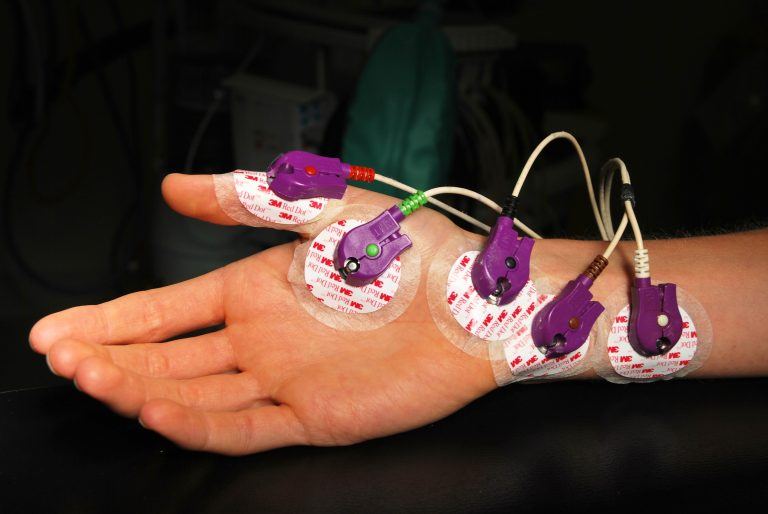
\includegraphics[width=0.4\textwidth]{./graphics/img-emg.jpg}
    \captionof{figure}{Elektroden voor Meting}
    \label{figure:emg}
\end{center}

\begin{center}
    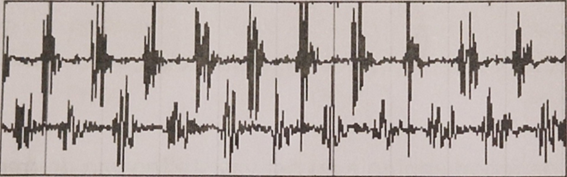
\includegraphics[width=0.4\textwidth]{./graphics/graph-emg.png}
    \captionof{figure}{Elektromyogram}
    \label{figure:emggraph}
\end{center}

Een EEG en een MEG zijn twee manieren om hersenactiviteit (encefalo) te beschrijven (grafie).
Dit kan worden gedaan door middel van elektriciteit (elektro) of door middel van magneten (magneto).
Het weten van de hersenactiviteit kan helpen met het bepalen welke soort tremor zich voordoet bij een patiënt \cite{elsevier2022,knf2022}.
De EEG is de meer gebruikelijke van de twee methoden en wordt vaak gebruikt in combinatie met een EMG \cite{knf2022}.
Vergelijkbaar met de EMG wordt elektrische activiteit, of hersengolven, gemeten met elektroden te zien in Figuur~\ref{figure:emg}.
Het resultaat van de meting is eveneens vergelijkbaar met dat van de EMG, en is te zien in Figuur~\ref{figure:emggraph}.

Een andere mogelijkheid is de fMRI \cite{elsevier2022}.
Hiermee kan er een 3D-weergave worden gemaakt van de hersenen.
Hierop is te zien waar en wanneer er activiteit plaatsvindt.
Dit wordt gedaan door het verschil tussen zuurstofarm en zuurstofrijk bloed weer te geven.
Dit kan gemeten worden door middel van het ijzer in het bloed \cite{hersenstichting2023}.

Tijdens het onderzoeken van iemands aandoening, wordt er soms gebruik gemaakt van hersenstimulaties.
Op deze manier kan er meer, en vaak beter, bewijs worden verzameld voor de diagnose van een aandoening \cite{elsevier2022}.

\subsection{Welke methodes zijn geschikt?}

Voor de rest van het onderzoek is het belangrijk om te bepalen wat de voorkeur aan detectiemethode wordt.
Deze keuze is gebaseerd op zowel de informatie die met de methode te verkrijgen is, als ook beschikbare tijd en kennis.

Met deze punten in het achterhoofd is de keuze geëindigd op de EMG.
De oorzaak van ET is onbekend, hierbij wordt er verwacht dat het vanuit de kleine hersenen komt \cite{elsevier2022}.
De hoeveelheid kennis die nodig is voor het interpreteren van hersenactiviteit is daarbij vele malen meer dan van een spieractiviteit.
Technologieën zoals draagbare EMG's maken het ook mogelijk om eventuele bevinden op dit gebied sneller op bruikbare schaal te krijgen \cite{frontiers2022}.
